
%%%%%%%%%%%%%%%%%%%%%%% file typeinst.tex %%%%%%%%%%%%%%%%%%%%%%%%%
%
% This is the LaTeX source for the instructions to authors using
% the LaTeX document class 'llncs.cls' for contributions to
% the Lecture Notes in Computer Sciences series.
% http://www.springer.com/lncs       Springer Heidelberg 2006/05/04
%
% It may be used as a template for your own input - copy it
% to a new file with a new name and use it as the basis
% for your article.
%
% NB: the document class 'llncs' has its own and detailed documentation, see
% ftp://ftp.springer.de/data/pubftp/pub/tex/latex/llncs/latex2e/llncsdoc.pdf
%
%%%%%%%%%%%%%%%%%%%%%%%%%%%%%%%%%%%%%%%%%%%%%%%%%%%%%%%%%%%%%%%%%%%


\documentclass[runningheads,a4paper]{llncs}

\usepackage{amssymb}
\setcounter{tocdepth}{3}
\usepackage{graphicx}
\usepackage{cite}
\usepackage{url}
\urldef{\mailsa}\path|{samuel.neaves}@kcl.ac.uk|

   
\newcommand{\keywords}[1]{\par\addvspace\baselineskip
\noindent\keywordname\enspace\ignorespaces#1}

\begin{document}

\mainmatter  % start of an individual contribution


\title{An Application of ILP to Systems Biology}
% oe Identifying Pathway Activation Patterns- For Classification
%ILP identifies pathway activation patterns. 
% a short form should be given in case it is too long for the running head
\titlerunning{Lecture Notes in Computer Science: Authors' Instructions}

% the name(s) of the author(s) follow(s) next
%
% NB: Chinese authors should write their first names(s) in front of
% their surnames. This ensures that the names appear correctly in
% the running heads and the author index.
%
\author{Samuel R Neaves}
%
\authorrunning{Lecture Notes in Computer Science: Authors' Instructions}
% (feature abused for this document to repeat the title also on left hand pages)

% the affiliations are given next; don't give your e-mail address
% unless you accept that it will be published
\institute{Deparment of Informatics King's College London,\\
Strand, London, UK\\
\mailsa\\
%\mailsc\\
\url{http://www.kcl.ac.uk}}

%
% NB: a more complex sample for affiliations and the mapping to the
% corresponding authors can be found in the file "llncs.dem"
% (search for the string "\mainmatter" where a contribution starts).
% "llncs.dem" accompanies the document class "llncs.cls".
%

\toctitle{Lecture Notes in Computer Science}
\tocauthor{Authors' Instructions}
\maketitle


\begin{abstract}
We show how a logical aggregation method combined 
with propositionalization methods can construct novel structured biological features for 	classification and ranking tasks in systems biology. 

\keywords{Biological Pathways, Reactome, RDF, Barcode, Logical Aggregation, Warmr, Treeliker, ILP.}
\end{abstract}


\section{Introduction and Background}

This paper describes a method to use Inductive Logic Programming(ILP) techniques to mine structured biological data. The biological problem addressed in this paper is the task of  understanding the system perturbations in different types of Lung Cancer; for details about the motivation of this task please see  ~\cite{Nobody06}.

A basic pipe line for this kind of task is to identify differentially expressed genes, and then in subsequent analysis look for how these genes may be related and subject them to further research.  Alternatively the task can be formalised as a classification task (of samples) or more generally as a ranking task. Remembering that classification is often not the true task -The classification performance is used as a measure of the quality of the identified differences. Classification might not be the true task as the class of a sample may already be known. (For example where the biopsy is taken from may indicate the class). When classification models are built it is common for this to be done using an attribute value representation where samples are vectors of gene expressions. The researchers are interested in the genes that are most important in the constructed model. Genes that are identified in this manner may be  different to a simple list of differently expressed genes as the constructed model may have found dependencies on genes which are not highly differently expressed. 

Whether researchers have identified a list of genes through differential expression analysis or by taking top features from a classification model, they have yet to take into account known relations between the genes. Therefore  a common next step is for researchers to look for connections between these genes, for example by performing Gene Set Enrichment Analysis(GSEA). These gene sets define a relation between the genes,  examples of gene sets include: functionally defined sets, cellular location defined sets, pathway defined sets, or network defined topological sets (These can be identified by community detection in a gene-network).

Past ILP research has integrated the two steps of finding differently expressed genes and GSEA by using relational subgroup discovery. These have used the hierarchical Gene Ontology to relate genes and has the advantage of being able to construct novel sets by sharing variables across predicates that define the set. Other ways researchers have tried to use known relations include simple attempts to aggregate across the set of genes by taking an average expression or other measure such as the SVD, see X for a review of these methods.  In most of these methods it is common to ignore the detailed relations between entities in a pathway, the pathway is treated as an unstructured collection of genes. Only do topologically defined sets take advantage of any known internal relations. But often these create crude clusters of genes, and do not follow biological intuition of information flow through the pathway.In addition the chosen network representation is often inappropriate for pathway analysis because of the problem discussed in [X].

Therefore a major limitation of the current approaches is that the models constructed are limited to being constructed from either genes or crude aggregates of sets of genes. But biological researchers are not only interested in lists of genes expression difference and how those genes in particular relate. More general pathway activation patterns are also of interest. Two examples are consistency modelling and network motif finding.
In consistency modelling the pattern depicted in figure 1 is matched against gene regulatory networks to check for consistency and Answer Set Programming techniques are used to amend the pathways to remove the inconsistency. Similar work has been done in ILP where biological pathways have been constructed and amended. 
 
In conventional network motif finding, again the biological intuition of information flow is ignored and it uncommon to either take into account the class of the network sample or to include uninstantiated variables in the search for patterns. 

In contrast to the work on consistency modelling, in this work we assume the pathways are in some sense correct and we are looking at individuals samples expression patterns mapped on to the network. This work is most similar to  "Using Bio-Pathways in Relational Learning 2008" where the authors propose using fully coupled fluxes. An FCF is the longest possible chain of vertices in which non-zero vertex activation implies a certain (non-zero) activation in its successors.

\section{Aim}
The aim is to identify pathway activation patterns that differ between biological samples, in order to give a biologist more information. This is achieved by using structural pathway information to build first order features that can be used to construct classification and ranking models, which will provide an appropriate level of abstraction for the interpretation of the model to be insightful for a biologist. 

	  
\section{Method}
\subsection{GEO Data}
GSE2109. This has 38 SCC and 33 AC Samples. 
	
\subsection{Biological Pathway Data}
Reactome is a collection of manually curated peer reviewed pathways. Reactome is made available as an RDF Xml Biopax level 3 file. This allows for simple passing using SWI-Prolog's semantic web libraries. 
In this work we use a high level logical abstraction of the idea of a biological pathway. In biological research it is common to see many types of biological networks represented by mathematical graphs. When considering biological pathways simple directed networks of genes and proteins are not appropriate, because this formalism does not adequately model the dependencies of activation patterns- either bipartite graphs or hypergraphs are required. We address this problem by using a directed reaction centric graph extracted from Reactome. In this way we address the problem identified in X.  Boolean networks are a common abstraction, but these are normally applied at the gene or protein level not at the reaction level. To use a boolean network abstraction on a reaction network, we apply a logical aggregation method from the measured probes in the microarray to reactions as defined in Reactome. 
\subsection{Barcode}
The first step is to binarize the probe values.Barcode is a tool for applying learnt thresholds to microarray data. This gives a binary value for each probe in the microarray. This tool is implemented as a R package.
\subsection{Logical Aggregation} 
Once we have binary probe values, we can use the structure provided by
the Reactome RDF graphs and our biological understanding to build Reaction level features.
 
Reactom defines reactions with entities, substrates, enzymes and products.
Each reaction has a set of inputs and set of outputs, in addition a reaction may be controlled(activated or inhibited) by an entity. 
Entities in Reactome include protein complexes and sets. 
A protein complex or protein set may itself include lower complexes or sets. This gives the input to a reaction a kind of tree structure. For the logical aggregation step we interpret this structure as a simple logical circuit. There can be a many to many relation between probes and proteins. 

In this way we can say that a reaction 'can proceed' if and only if, the input circuit evaluates to true. If a reaction 'can proceed' then we say that it is 'on' otherwise we say that it is 'off'. 
\subsection{Network Extraction}
Linking Reaction Removing trivial entities.
\subsection{Propositionalization}
It has been recommend to try prop methods first when attempting ILP
\subsubsection{Warmr}
Warmr is the first order equivalent of item set and association rule mining.It can be used as propositionalization method by searching for frequent queries in the two classes, and taking the set difference (not sure if this would work). An advantage of using Warmr is that it is easy to define background predicates for relevant concepts. For example a path or loop of all 'on' reactions. As Warmr does not prune by classification it however can quickly build to an intractable search with many irrelevant or similar queries/features built. 
	     
\subsubsection{Tree Liker}
Tree liker is a modern ILP tool that implements a number of algorithms it has been shown to produce long features, by building features bottom up in blockwise manner. This is a desirable trait for  this task as longer features will give more information to a biologist. A limitation is that the features are 'tree like' which means there can be no cycles in the variables. 
Treeliker does not require a variable for the sample as this is done automatically. Treeliker unlike Warmr does not support explicit background knowledge and therefore all relevant relations need to be preprocessed using prolog.
 
\noindent
%\it{Illustrative Tree Liker Template}
\begin{verbatim}
  set(output_type,single)
  set(examples,'Pathway963.txt')
  set(template,[reaction(-R1,#onoroff),link(+R1,-R2,!T1),
   reaction(+R2,#onoroff),link(+R2,-R3,!T2),reaction(+R3,#onorff),
   link(!RA,-R4,!T3),link(+R4,!RB,!T4),link(+R1,-R2,#T1),
   link(+R2,-R3,#T2),link(!RA,-R4,#T3),link(+R4,!RB,#T4)])
  set(output, Pathway963.arff)
  work(yes)
\end{verbatim}

\noindent
%\it{Example Tree Liker found feature}
\begin{verbatim}
  reaction(A, 0), link(A, B, follows), reaction(B, 1), link(B, C, _),    
  reaction(C, 0), link(A, D, activation), reaction(D, 0).
\end{verbatim}



\subsubsection{Combined Search}
	     
\subsection{Ranking and Classification}
As we are interested in producing comprehensible models, we limit our experiments to rule and tree building algorithms.We use 
\subsubsection{Appropriate Metrics}
Dream challenge uses the following metrics
Flach et al recommend these metrics. 
	     
\section{Results}
ROC curve
Features Found and models built.
\section{Discussion}
This work has shown the appropriateness of using ILP methods to mine the abundance of highly structured biological data.Using this method we have identified differences in pathway activation patterns that go beyond the standard analysis of differentially expressed genes, enrichment analysis, gene feature ranking and pattern mining for common network motifs (by using pre-defined background knowledge predicate in Warmr such as onpath. The use of logical aggregation to a  reaction graph simplifies the search for hypothesises to an extent where all pathways can be searched in reasonable time. The extension of Treeliker found features with Warmr to connect loops is believed to be novel. This allows for the finding of loops with additional properties in a reasonable amount of time.  



\subsection{Additional Information Required by the Volume Editor}

If you have more than one surname, please make sure that the Volume Editor
knows how you are to be listed in the author index.




Please do
\emph{not} change the preset fonts. If you have to use fonts other
than the preset fonts, kindly submit these with your files.

Please use the commands \verb+\label+ and \verb+\ref+ for
cross-references and the commands \verb+\bibitem+ and \verb+\cite+ for
references to the bibliography, to enable us to create hyperlinks at
these places.

For preparing your figures electronically and integrating them into
your source file we recommend using the standard \LaTeX{} \verb+graphics+ or
\verb+graphicx+ package. These provide the \verb+\includegraphics+ command.
In general, please refrain from using the \verb+\special+ command.

Remember to submit any further style files and
fonts you have used together with your source files.

\subsubsection{Headings.}

Headings should be capitalized
(i.e., nouns, verbs, and all other words
except articles, prepositions, and conjunctions should be set with an
initial capital) and should,
with the exception of the title, be aligned to the left.
Words joined by a hyphen are subject to a special rule. If the first
word can stand alone, the second word should be capitalized.

Here are some examples of headings: ``Criteria to Disprove
Context-Freeness of Collage Language", ``On Correcting the Intrusion of
Tracing Non-deterministic Programs by Software", ``A User-Friendly and
Extendable Data Distribution System", ``Multi-flip Networks:
Parallelizing GenSAT", ``Self-determinations of Man".

\subsubsection{Lemmas, Propositions, and Theorems.}

The numbers accorded to lemmas, propositions, and theorems, etc. should
appear in consecutive order, starting with Lemma 1, and not, for
example, with Lemma 11.

\subsection{Figures}

For \LaTeX\ users, we recommend using the \emph{graphics} or \emph{graphicx}
package and the \verb+\includegraphics+ command.

Please check that the lines in line drawings are not
interrupted and are of a constant width. Grids and details within the
figures must be clearly legible and may not be written one on top of
the other. Line drawings should have a resolution of at least 800 dpi
(preferably 1200 dpi). The lettering in figures should have a height of
2~mm (10-point type). Figures should be numbered and should have a
caption which should always be positioned \emph{under} the figures, in
contrast to the caption belonging to a table, which should always appear
\emph{above} the table; this is simply achieved as matter of sequence in
your source.

Please center the figures or your tabular material by using the \verb+\centering+
declaration. Short captions are centered by default between the margins
and typeset in 9-point type (Fig.~\ref{fig:example} shows an example).
The distance between text and figure is preset to be about 8~mm, the
distance between figure and caption about 6~mm.

To ensure that the reproduction of your illustrations is of a reasonable
quality, we advise against the use of shading. The contrast should be as
pronounced as possible.

If screenshots are necessary, please make sure that you are happy with
the print quality before you send the files.
\begin{figure}
\centering
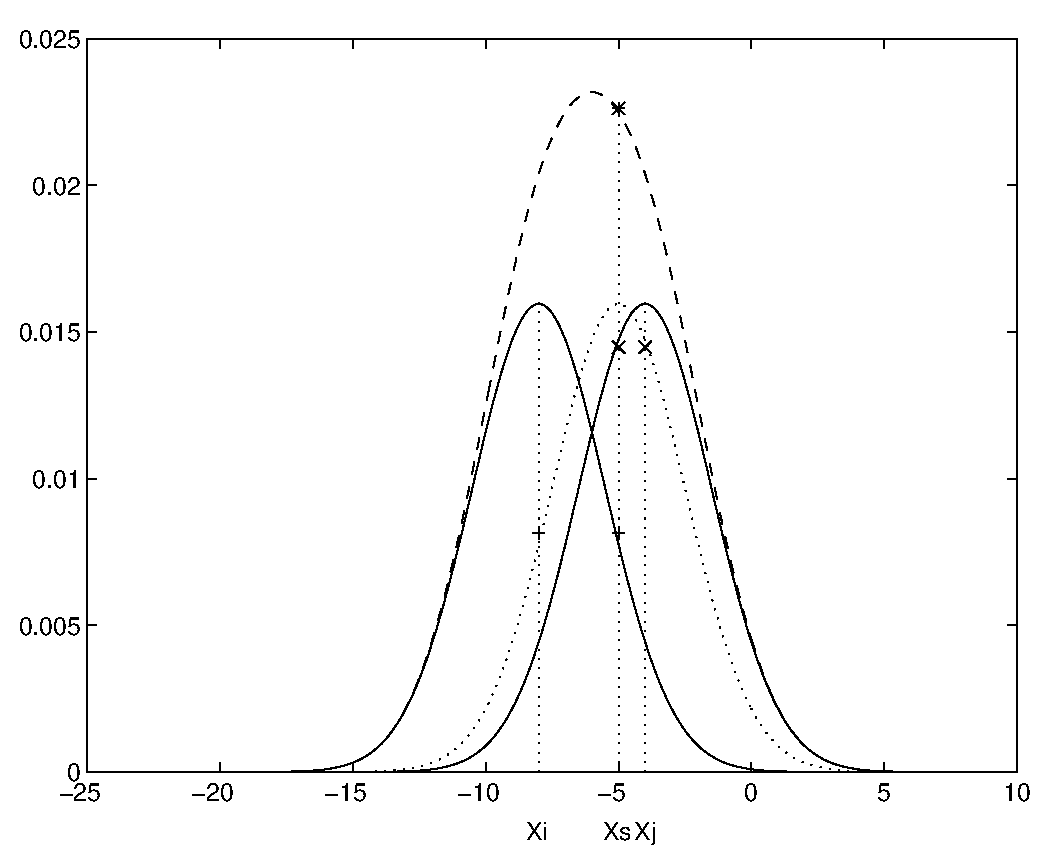
\includegraphics[height=6.2cm]{eijkel2}
\caption{One kernel at $x_s$ (\emph{dotted kernel}) or two kernels at
$x_i$ and $x_j$ (\textit{left and right}) lead to the same summed estimate
at $x_s$. This shows a figure consisting of different types of
lines. Elements of the figure described in the caption should be set in
italics, in parentheses, as shown in this sample caption.}
\label{fig:example}
\end{figure}

Please define figures (and tables) as floating objects. Please avoid
using optional location parameters like ``\verb+[h]+" for ``here".

\paragraph{Remark 1.}

In the printed volumes, illustrations are generally black and white
(halftones), and only in exceptional cases, and if the author is
prepared to cover the extra cost for color reproduction, are colored
pictures accepted. Colored pictures are welcome in the electronic
version free of charge. If you send colored figures that are to be
printed in black and white, please make sure that they really are
legible in black and white. Some colors as well as the contrast of
converted colors show up very poorly when printed in black and white.

\subsection{Formulas}

Displayed equations or formulas are centered and set on a separate
line (with an extra line or halfline space above and below). Displayed
expressions should be numbered for reference. The numbers should be
consecutive within each section or within the contribution,
with numbers enclosed in parentheses and set on the right margin --
which is the default if you use the \emph{equation} environment, e.g.,
\begin{equation}
  \psi (u) = \int_{o}^{T} \left[\frac{1}{2}
  \left(\Lambda_{o}^{-1} u,u\right) + N^{\ast} (-u)\right] dt \;  .
\end{equation}

Equations should be punctuated in the same way as ordinary
text but with a small space before the end punctuation mark.

\subsection{Footnotes}

The superscript numeral used to refer to a footnote appears in the text
either directly after the word to be discussed or -- in relation to a
phrase or a sentence -- following the punctuation sign (comma,
semicolon, or period). Footnotes should appear at the bottom of
the
normal text area, with a line of about 2~cm set
immediately above them.\footnote{The footnote numeral is set flush left
and the text follows with the usual word spacing.}

\subsection{Program Code}

Program listings or program commands in the text are normally set in
typewriter font, e.g., CMTT10 or Courier.

\medskip

\noindent
{\it Example of a Computer Program}
\begin{verbatim}
program Inflation (Output)
  {Assuming annual inflation rates of 7%, 8%, and 10%,...
   years};
   const
     MaxYears = 10;
   var
     Year: 0..MaxYears;
     Factor1, Factor2, Factor3: Real;
   begin
     Year := 0;
     Factor1 := 1.0; Factor2 := 1.0; Factor3 := 1.0;
     WriteLn('Year  7% 8% 10%'); WriteLn;
     repeat
       Year := Year + 1;
       Factor1 := Factor1 * 1.07;
       Factor2 := Factor2 * 1.08;
       Factor3 := Factor3 * 1.10;
       WriteLn(Year:5,Factor1:7:3,Factor2:7:3,Factor3:7:3)
     until Year = MaxYears
end.
\end{verbatim}
%
\noindent
{\small (Example from Jensen K., Wirth N. (1991) Pascal user manual and
report. Springer, New York)}

\subsection{Citations}

For citations in the text please use
square brackets and consecutive numbers: \cite{jour}, \cite{lncschap},
\cite{proceeding1} -- provided automatically
by \LaTeX 's \verb|\cite| \dots\verb|\bibitem| mechanism.

\subsection{Page Numbering and Running Heads}

There is no need to include page numbers. If your paper title is too
long to serve as a running head, it will be shortened. Your suggestion
as to how to shorten it would be most welcome.

\section{LNCS Online}

The online version of the volume will be available in LNCS Online.
Members of institutes subscribing to the Lecture Notes in Computer
Science series have access to all the pdfs of all the online
publications. Non-subscribers can only read as far as the abstracts. If
they try to go beyond this point, they are automatically asked, whether
they would like to order the pdf, and are given instructions as to how
to do so.

Please note that, if your email address is given in your paper,
it will also be included in the meta data of the online version.

\section{BibTeX Entries}

The correct BibTeX entries for the Lecture Notes in Computer Science
volumes can be found at the following Website shortly after the
publication of the book:
\url{http://www.informatik.uni-trier.de/~ley/db/journals/lncs.html}

\subsubsection*{Acknowledgments.} The heading should be treated as a
subsubsection heading and should not be assigned a number.

\section{The References Section}\label{references}

In order to permit cross referencing within LNCS-Online, and eventually
between different publishers and their online databases, LNCS will,
from now on, be standardizing the format of the references. This new
feature will increase the visibility of publications and facilitate
academic research considerably. Please base your references on the
examples below. References that don't adhere to this style will be
reformatted by Springer. You should therefore check your references
thoroughly when you receive the final pdf of your paper.
The reference section must be complete. You may not omit references.
Instructions as to where to find a fuller version of the references are
not permissible.

We only accept references written using the latin alphabet. If the title
of the book you are referring to is in Russian or Chinese, then please write
(in Russian) or (in Chinese) at the end of the transcript or translation
of the title.

The following section shows a sample reference list with entries for
journal articles \cite{jour}, an LNCS chapter \cite{lncschap}, a book
\cite{book}, proceedings without editors \cite{proceeding1} and
\cite{proceeding2}, as well as a URL \cite{url}.
Please note that proceedings published in LNCS are not cited with their
full titles, but with their acronyms!


\bibliography{mybib}{}
\bibliographystyle{plain}

\begin{thebibliography}{4}

\bibitem{jour} Smith, T.F., Waterman, M.S.: Identification of Common Molecular
Subsequences. J. Mol. Biol. 147, 195--197 (1981)

\bibitem{lncschap} May, P., Ehrlich, H.C., Steinke, T.: ZIB Structure Prediction Pipeline:
Composing a Complex Biological Workflow through Web Services. In: Nagel,
W.E., Walter, W.V., Lehner, W. (eds.) Euro-Par 2006. LNCS, vol. 4128,
pp. 1148--1158. Springer, Heidelberg (2006)

\bibitem{book} Foster, I., Kesselman, C.: The Grid: Blueprint for a New Computing
Infrastructure. Morgan Kaufmann, San Francisco (1999)

\bibitem{proceeding1} Czajkowski, K., Fitzgerald, S., Foster, I., Kesselman, C.: Grid
Information Services for Distributed Resource Sharing. In: 10th IEEE
International Symposium on High Performance Distributed Computing, pp.
181--184. IEEE Press, New York (2001)

\bibitem{proceeding2} Foster, I., Kesselman, C., Nick, J., Tuecke, S.: The Physiology of the
Grid: an Open Grid Services Architecture for Distributed Systems
Integration. Technical report, Global Grid Forum (2002)

\bibitem{url} National Center for Biotechnology Information, \url{http://www.ncbi.nlm.nih.gov}

\end{thebibliography}


\section*{Appendix: Springer-Author Discount}

LNCS authors are entitled to a 33.3\% discount off all Springer
publications. Before placing an order, the author should send an email, 
giving full details of his or her Springer publication,
to \url{orders-HD-individuals@springer.com} to obtain a so-called token. This token is a
number, which must be entered when placing an order via the Internet, in
order to obtain the discount.

\section{Checklist of Items to be Sent to Volume Editors}
Here is a checklist of everything the volume editor requires from you:


\begin{itemize}
\settowidth{\leftmargin}{{\Large$\square$}}\advance\leftmargin\labelsep
\itemsep8pt\relax
\renewcommand\labelitemi{{\lower1.5pt\hbox{\Large$\square$}}}

\item The final \LaTeX{} source files
\item A final PDF file
\item A copyright form, signed by one author on behalf of all of the
authors of the paper.
\item A read me giving the name and email address of the
corresponding author.
\end{itemize}
\end{document}
